\section{Grundlagen}
Im folgenden werden verschiedene Grundlagen ausgef\"uhrt.

\subsection{Elektromagnetische Grundgleichungen}
Die Theorie der magnetischen und auch elektromegnetischen Felder basiert im allgemeinen auf den Maxwell Gleichungen~\cite{maxwell1865viii}. Diese lauten:
\begin{align}
	\rot \vec{E} &= -\pet \vec{B} \\
	\dive \vec{D} &= \rho \\
	\rot \vec{H} &= \vec{J} + \pet\vec{D} \label{eq:max3} \\
	\dive \vec{B} &= 0 \label{eq:max4}
\end{align}
\par
Die Variablen entsprechen dabei:
\begin{itemize}
	\item $\vec{E}$: Elektrische Feldst\"arke
	\item $\vec{D}$: Elektrische Flussdichte
	\item $\vec{H}$: Magnetische Feldst\"arke
	\item $\vec{B}$: Magnetische Flussdichte
	\item $\vec{J}$: Elektrische Stromdichte
	\item $\rho$ Ladungsdichte
\end{itemize}
\par
F\"ur unsere Herleitung sind in erster Linie die Gleichungen~\ref{eq:max3} und~\ref{eq:max4} relevant. F\"ur die Statische Betrahtung verschwinden zus\"atzlich die enthaltenen Zeitableitungen, sodass sich~\ref{eq:max3} vereinfacht zu:
\begin{equation}
	\rot \vec{H} = \vec{J}
	\label{eq:amplaw}
\end{equation}
\par
Diese Sonderform der 3. Maxwellschen Gleichung wird auch das Amperesche Gesetz der Magnetostatik genannt.
\par
Dar\"uber hinaus werden noch Materialbeziehungen ben\"otigt. Diese stellen eine Beziehung zwischen den Feldst\"arken und den Flussdichten her~\cite{maxwell1865viii}.
\begin{align}
	\vec{B} &= \mu\vec{H} \\
	\vec{D} &= \epsilon\vec{E} \\
	\vec{J} &= \kappa\vec{E}
\end{align}
\par
Die Permittivit\"at $\epsilon$, Permeabilität $\mu$ und Leitf\"ahigkeit $\kappa$ stellen dabei die Kopplungsgr\"o\ss{}en dar.

\subsection{Vektoranalytische Grundgleichungen}
Zur Herleitung der gew\"unschten Formulierung werden zus\"atzlich mehrere Gleichungen aus der Vektoranalysis ben\"otigt. Diese besagen folgendes.
\par
Ein Wirbelfeld ist immer Divergenzfrei:
\begin{equation}
	\dive\rot \vec{u} = 0
	\label{eq:divfree}
\end{equation}
\par
Ein Quellenfeld ist Wirbelfrei:
\begin{equation}
	\rot \grad\Phi = 0
\end{equation}
Der Wirbel eines Wirbels l\"asst sich aufteilen:
\par
\begin{equation}
	\rot\rot \vec{u} = \grad\dive \vec{u} - \Delta \vec{u}
\end{equation}

\subsection{De-Rham-Komplex}
Die eingef\"uhrten Grundgleichungen lassen sich auch in einen Komplex \"uberf\"uhren. Die genauen Funktionenr\"aume, werden sp\"ater noch eingef\"uhrt.
\begin{figure}[!h]
	\centering
	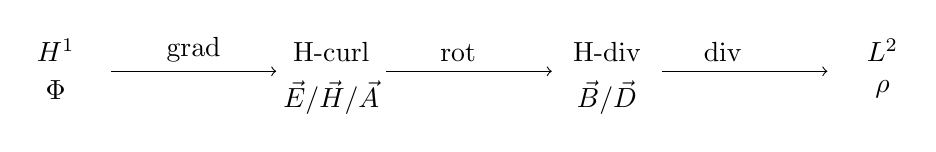
\begin{tikzpicture}[scale=2.8]

	\draw[->] (0.25,1) -- (1,1);
	\draw[->] (1.5,1) -- (2.25,1);
	\draw[->] (2.75,1) -- (3.5,1);

	\node at (0.625,1) [above] {grad};
	\node at (1.825,1) [above] {rot};
	\node at (3.025,1) [above] {div};

	\node at (0,1) [above] {$H^1$};
	\node at (0,1) [below] {$\Phi$};
	\node at (1.25,1) [below] {$\vec{E}$/$\vec{H}$/$\vec{A}$};
	\node at (1.25,1) [above] {H-curl};
	\node at (2.5,1) [above] {H-div};
	\node at (2.5,1) [below] {$\vec{B}$/$\vec{D}$};
	\node at (3.75,1) [above] {$L^2$};
	\node at (3.75,1) [below] {$\rho$};
	\end{tikzpicture}
\end{figure}
Es l\"asst sich zeigen, dass auf einfach zusammenhängenden Gebieten ein Operator in dieser Sequenz exakt dem Kern des nächsten Operators entspricht.

